\subsection{\CVCV doesn't capture \emph{schwa never word-initial}}
No explanation for \enquote{schwa never word-initial} if schwa does govern,
The structure below of a word starting with Schwa is perfectly
fine in \CVCV.

This configuration however is consistently absent in German,
which indicates that there might be a \tr{tiefergehender Zusammenhang}
that \CVCV doesn't manage to capture.

\begin{structure}{}
  \drawCV{1}
  \wordstart
  \C{\ti P}
  \V{\schwaCons}
\end{structure}

\cite[p.~650]{scheer2004}
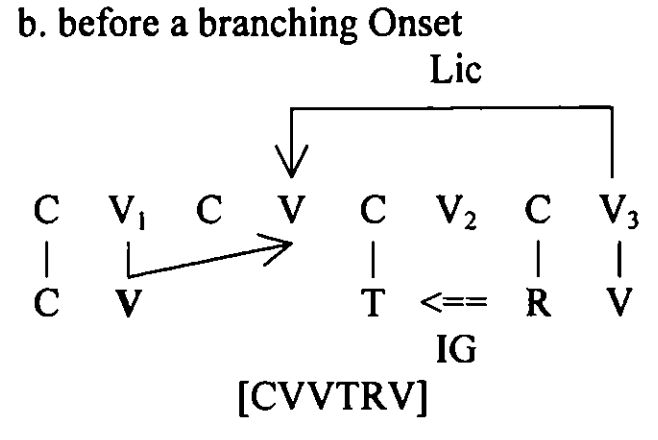
\includegraphics[width=.5\textwidth]{figures/lic-over-branching-onset.png}
\\If $V_3$ licenses long vowel, how can IG be allowed?